\documentclass[]{homework}
\usepackage{amsmath}
\usepackage{wrapfig}

\begin{document}


\exam{1}{Feb. 26, 2021}

  \noindent\textbf{Read the following.} It contains important information
  about this exam.

  \begin{itemize}
    \item You must submit your solutions
    to Canvas \textbf{by 4:00 pm}! Please plan accordingly.
    This gives you approximately 1.5 hours for this exam.
    \item There is both a written and computational part to this exam. You
    will need to download both from Canvas, and submit solutions for both to Canvas.
    \item You are allowed to use any reference materials you like for this
      exam, except each other.
    \item You should make an effort to answer all questions on this exam.
      Clearly identify your final answers, and clearly explain your solutions.
      This will be graded according to the syllabus rubric, so effort will be
      heavily weighted.
  \end{itemize}



\begin{problem}{1}
  Clearly explain your answers to the following questions.
  \begin{subproblem}{a}
    Mathematically the equation $x+h=x$ has the unique solution $h=0$.
    Numerically this statement can be true even if $h\ne0$.
    Explain how this can occur.
  \end{subproblem}
  \begin{subproblem}{b}
    When using a root finding algorithm such as \code{scipy.optimize.brentq()} we are forced bracket the root.
    This can seem like an annoying and tedious requirement.
    Why is it (almost) always best to use an algorithm that requires bracketing?
  \end{subproblem}
  \begin{subproblem}{c}
    The Newton-Raphson method for finding roots uses the first derivative of the function and does \emph{not require} bracketing!
    Briefly discuss when/why this can still be a good method for finding roots.
  \end{subproblem}
\end{problem}

\begin{problem}{2}
  When working with functions numerically,
  we often only know values of a
        function $f(x)$ at
      discrete locations. We have seen that we can fit polynomials or splines

    \begin{minipage}[t]{\linewidth}
      \vspace{-1.4  em}
      \begin{wrapfigure}{r}{2.0in}
        \vspace{-1.5em}
        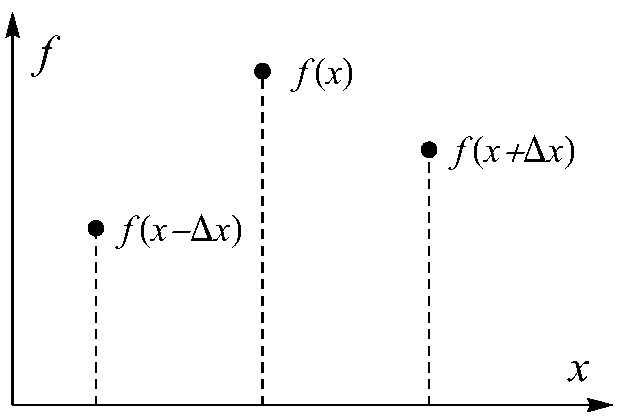
\includegraphics[width=2.0in]{examfig.pdf}
      \end{wrapfigure}
      to sets of points
      in order to interpolate between the points. We are also often interested in computing
      derivatives of functions, and need to come up with approximate ways of doing so.
      Below we explore three different options for determining the derivative $f'(x)$, given
      knowledge of $f(x)$ at three regularly spaced points as shown in the figure to the right.
    \end{minipage}

  \begin{subproblem}{a}
    One method for approximating a function involves looking at its Taylor series expansion.
    Write down the second-order Taylor series expansion of $f(x)$ at the
    points $x+\Delta x$ and $x-\Delta x$, that is, compute the expansions of $f(x+\Delta x)$ and $f(x-\Delta x)$.
    Combine these expressions to eliminate the second derivative, $f''(x)$,
    and determine an approximate formula for $f'(x)$.
  \end{subproblem}
  \begin{subproblem}{b}
    We can also determine the unique quadratic polynomial that
    intersects all three points,
    \[
      f_{\rm poly}(x) = a x^2 + bx + c\,,
    \]
    And evaluate its derivative.
    First, notice that we want $f_{\rm poly} = f$ at each point.
    Provide an expression for the derivative at the point $x$, $f_{\rm poly}'(x)$,
    in terms of the quantities $f(x-\Delta x)$, $f(x)$, $f(x+\Delta x)$, and $\Delta x$.

    \hint{You can solve for the coefficients $a$ and $b$, but finding $c$ is not necessary.
    You can also take advantage of your result from part a) of this question!}
  \end{subproblem}
  \begin{subproblem}{c}
    A final method is to consider what happens when we fit a linear function to these three points.
    In class, we derived down analytic expressions for the coefficients of a
    linear fit. For the line $f_{\rm lin}(x) = a + b x$, the expression for the slope of the
    line was given by
    \[
      b = \frac{S S_{xf} - S_x S_f}{S S_{xx} - S_x^2}\,,
    \]
    where the $S$ parameters were uncertainty-weighted averages. Here we will assume
    the uncertainties are all identical, allowing us to use the following expressions:
    \begin{align*}
      S  & = \sum_i 1  & S_{x} & = \sum_i x^i     & S_{xf} & = \sum_i x^i f(x^i) \\
         &             & S_{f} & = \sum_i f(x^i)  & S_{xx} & = \sum_i (x^i)^2\,.
    \end{align*}
    Using these expressions, determine the coefficient $b$, and thereby an approximation for the
    derivative, $f'(x) \simeq f'_{\rm lin}(x) = b$.
  \end{subproblem}

\end{problem}


\end{document}

